% Created: 12-FEB-2021
% Revised: 
%
% VERSION 0.1
%
\documentclass{article}

\usepackage{graphicx} % screenshots
\usepackage{fancyhdr} % Required for custom headers
\usepackage{lastpage} % Required to determine the last page for the footer
\usepackage{extramarks} % Required for headers and footers
\usepackage{paralist} % compact lists
\usepackage{parskip} % more space between paragraphs
\usepackage{textcomp} % straight quotes for code
\usepackage{hyperref} % for hyperlinks in the document
\usepackage{tabularx} % for text-wrapping in tables
\usepackage{algorithm} % algorithms
\usepackage{algpseudocode} % algorithms
\usepackage{fancyvrb} % for nice examples
\usepackage{tikz} % diagrams

% Set up Tikz Library
\usetikzlibrary{shapes.geometric}
\usetikzlibrary{shapes.multipart}
\usetikzlibrary{positioning}
\usetikzlibrary{arrows}
\usetikzlibrary{arrows.meta}
\usetikzlibrary{fit}
\usetikzlibrary{matrix}
\usetikzlibrary{shadows}
\usetikzlibrary{calc}

% Primary key should be underlined
\newcommand{\primarykey}[1]{\underline{#1}}

%%%%% ENTITY %%%%%%

% Entity - Basic rect
\tikzstyle{entity} = [rectangle, draw, thick, black, minimum width=4em, minimum height=2.5em]

% Weak Entity - Double lined rect
\tikzstyle{weak entity} = [entity, double, double distance=2pt]

%%%%% Attribute %%%%%%

% Attribute - Ellipse around attribute
\tikzstyle{attribute} = [ellipse, draw, black, thick, minimum width=5em, minimum height=2em]

% Multi-value attribute - double circled ellipse
\tikzstyle{multi attribute} = [attribute, double, double distance=2pt]

% Derived attribute - Dashed ellipse
\tikzstyle{derived attribute} = [attribute, dashed]

%%%%% Relationship %%%%%%

% Relationship - diamond
\tikzstyle{relationship} = [diamond, draw, black, thick, minimum width=2em, aspect=1, fill=white]

% Weak Entity Relationship - double diamond
\tikzstyle{weak relationship} = [relationship, double, double distance=2pt]

% IS-A relationship - triangle
\tikzstyle{isa} = [isosceles triangle, isosceles triangle apex angle=60, shape border rotate=120, draw, black, thick, minimum size=3em]

%%% Arrow style

\tikzstyle{oneone} = [-{Latex[width=10mm, length=10mm]}, line width=0.2cm]
\tikzstyle{zeroone} = [-{Latex[width=5mm, length=7mm]}]
\tikzstyle{zeromany} = [--]
\tikzstyle{onemany} = [--, line width=0.2cm]


%%% Crow Foot ERD style - PREFIX with ``cf'' %%%


%
% Crow Foot Many
%

\pgfarrowsdeclare{cfmany}{cfmany}
{
  \pgfarrowsleftextend{+-.5\pgflinewidth}%
  \pgfarrowsrightextend{+.5\pgflinewidth}%
}
{
  %\pgfutil@tempdima=0.6pt%
  %\advance\pgfutil@tempdima by.25\pgflinewidth%
  \pgfsetdash{}{+0pt}%
  \pgfsetmiterjoin%
  %\pgfpathmoveto{\pgfqpoint{0pt}{-9\pgfutil@tempdima}}%
  %\pgfpathlineto{\pgfqpoint{-13\pgfutil@tempdima}{0pt}}%
  %\pgfpathlineto{\pgfqpoint{0pt}{9\pgfutil@tempdima}}%
  %\pgfpathmoveto{\pgfqpoint{0\pgfutil@tempdima}{0\pgfutil@tempdima}}%
  \pgfpathmoveto{\pgfqpoint{-15pt}{-6pt}}% 
  \pgfpathlineto{\pgfqpoint{-15pt}{-6pt}}%  
  \pgfpathlineto{\pgfqpoint{-15pt}{6pt}}% 
  \pgfusepathqstroke%
}

%
% Crow Foot zero-Many
%

\pgfarrowsdeclare{cfomany}{cfomany}
{
  \pgfarrowsleftextend{+-.5\pgflinewidth}%
  \pgfarrowsrightextend{+.5\pgflinewidth}%
}
{
  %\pgfutil@tempdima=0.6pt%
  %\advance\pgfutil@tempdima by.25\pgflinewidth%
  \pgfsetdash{}{+0pt}%
  \pgfsetmiterjoin%
  %\pgfpathmoveto{\pgfqpoint{0pt}{-9pt\pgfutil@tempdima}}%
  %\pgfpathlineto{\pgfqpoint{-13pt\pgfutil@tempdima}{0pt}}%
  %\pgfpathlineto{\pgfqpoint{0pt}{9pt\pgfutil@tempdima}}%
  %\pgfpathmoveto{\pgfqpoint{0pt\pgfutil@tempdima}{0pt\pgfutil@tempdima}}%  
  %\pgfpathmoveto{\pgfqpoint{0pt\pgfutil@tempdima}{0pt\pgfutil@tempdima}}%
	\pgfpathmoveto{\pgfqpoint{0pt}{-6pt}}%
  \pgfpathlineto{\pgfqpoint{-13pt}{0pt}}%
  \pgfpathlineto{\pgfqpoint{0pt}{6pt}}%
  %\pgfpathmoveto{\pgfqpoint{0pt\pgfutil@tempdima}{0pt\pgfutil@tempdima}}%  
  %\pgfpathmoveto{\pgfqpoint{0pt\pgfutil@tempdima}{0pt\pgfutil@tempdima}}%
	\pgfpathmoveto{\pgfqpoint{-6pt}{-6pt}}% 
    \pgfpathcircle{\pgfpoint{-16.5pt}{0pt}} {3.5pt}
  \pgfusepathqstroke%
}


%
% Crow Foot One
%

\pgfarrowsdeclare{cfone}{cfone}
{
  \pgfarrowsleftextend{+-.5\pgflinewidth}%
  \pgfarrowsrightextend{+.5\pgflinewidth}%
}
{
  %\pgfutil@tempdima=0.6pt%
  %\advance\pgfutil@tempdima by.25\pgflinewidth%
  \pgfsetdash{}{+0pt}%
  \pgfsetmiterjoin%
  %\pgfpathmoveto{\pgfqpoint{0\pgfutil@tempdima}{0\pgfutil@tempdima}}%
	%\pgfpathmoveto{\pgfqpoint{0.6pt}{0.6pt}}%
  \pgfpathmoveto{\pgfqpoint{-6pt}{-6pt}}% 
  \pgfpathlineto{\pgfqpoint{-6pt}{-6pt}}%  
  \pgfpathlineto{\pgfqpoint{-6pt}{6pt}}% 
  %\pgfpathmoveto{\pgfqpoint{0\pgfutil@tempdima}{0\pgfutil@tempdima}}%
	%\pgfpathmoveto{\pgfqpoint{0.6pt}{0.6pt}}%
  \pgfpathmoveto{\pgfqpoint{-8pt}{-6pt}}% 
  \pgfpathlineto{\pgfqpoint{-8pt}{-6pt}}%  
  \pgfpathlineto{\pgfqpoint{-8pt}{6pt}}%    
  \pgfusepathqstroke%
}

%
% Crow Foot zero-One
%

\pgfarrowsdeclare{cfoone}{cfoone}
{
  \pgfarrowsleftextend{+-.5\pgflinewidth}%
  \pgfarrowsrightextend{+.5\pgflinewidth}%
}
{
  \pgfutil@tempdima=0.6pt%
  %\advance\pgfutil@tempdima by.25\pgflinewidth%
  \pgfsetdash{}{+0pt}%
  \pgfsetmiterjoin%
  %\pgfpathmoveto{\pgfqpoint{0\pgfutil@tempdima}{0\pgfutil@tempdima}}%
  \pgfpathmoveto{\pgfqpoint{-6pt}{-6pt}}% 
  \pgfpathlineto{\pgfqpoint{-6pt}{-6pt}}%  
  \pgfpathlineto{\pgfqpoint{-6pt}{6pt}}% 
  %\pgfpathmoveto{\pgfqpoint{0\pgfutil@tempdima}{0\pgfutil@tempdima}}%
    \pgfpathcircle{\pgfpoint{-12.5pt}{0}} {3.5pt}
  \pgfusepathqstroke%
}

\tikzset{
    zig zag to/.style={
        to path={(\tikztostart) -| ($(\tikztostart)!#1!(\tikztotarget)$) |- (\tikztotarget)}
    },
    zig zag to/.default=0.5,
    cfone to cfone/.style={
        cfone-cfone, zig zag to
    },    
    cfone to cfmany/.style={
        cfone-cfmany, zig zag to,
    },
    cfone to cfomany/.style={
        cfone-cfomany, zig zag to
    },      
    cfmany to cfone/.style={
        cfmany-cfone, zig zag to
    },
    cfmany to cfmany/.style={
        cfmany-cfmany, zig zag to
    },
    cfonemany/.style={
        cfmany-, zig zag to
    },
    cf0many/.style={
        cfomany-, zig zag to
    },
    cfoneone/.style={
        cfone-, zig zag to
    },
    cf0one/.style={
        cfoone-, zig zag to
    }
}
\def\property#1{\node[name=\entityname-#1, every property/.try]{#1};}
\def\properties{\begingroup\catcode`\_=11\relax\processproperties}
\def\processproperties#1{\endgroup%
    \def\propertycode{}%
    \foreach \p in {#1}{%
        \expandafter\expandafter\expandafter\gdef\expandafter\expandafter\expandafter\propertycode%
            \expandafter\expandafter\expandafter{\expandafter\propertycode\expandafter\property\expandafter{\p}\\}%
    }%
    \propertycode%
}

\tikzset{%
    pics/entity/.style n args={3}{code={%
        \node[draw,
        rectangle split,
        rectangle split parts=2,
        text height=1.5ex,
        ] (#1)
        {#2 \nodepart{second}
            \begin{tabular}{>{\raggedright\arraybackslash}p{6em}}
                #3
            \end{tabular}
        };%
    }}
}

\hypersetup{
    colorlinks=true
}

% Set up the header and footer
\pagestyle{fancy}
\lhead{\hmwkAuthorName} % Top left header
\chead{\hmwkTitle} % Top center head
\rhead{\hmwkClass} % Top right header
\lfoot{\lastxmark} % Bottom left footer
\cfoot{} % Bottom center footer
\rfoot{Page\ \thepage\ of\ \protect\pageref{LastPage}} % Bottom right footer
\renewcommand\headrulewidth{0.4pt} % Size of the header rule
%\renewcommand\footrulewidth{0.4pt} % Size of the footer rule

\setlength\parindent{0pt} % Removes all indentation from paragraphs

%----------------------------------------------------------------------------------------
%	DOCUMENT STRUCTURE COMMANDS
%	Skip this unless you know what you're doing
%----------------------------------------------------------------------------------------

% Header and footer for when a page split occurs within a problem environment
\newcommand{\enterProblemHeader}[1]{
% \nobreak\extramarks{#1}{#1 continued on next page\ldots}\nobreak
% \nobreak\extramarks{}{#1 continued on next page\ldots}\nobreak
}

% Header and footer for when a page split occurs between problem environments
\newcommand{\exitProblemHeader}[1]{
% \nobreak\extramarks{#1 (continued)}{#1 continued on next page\ldots}\nobreak
\nobreak\extramarks{#1}{}\nobreak
}

\setcounter{secnumdepth}{0} % Removes default section numbers
\newcounter{homeworkProblemCounter} % Creates a counter to keep track of the number of problems

\newcommand{\homeworkProblemName}{}
\newenvironment{homeworkProblem}[1][Problem \arabic{homeworkProblemCounter}]{ % Makes a new environment called homeworkProblem which takes 1 argument (custom name) but the default is "Problem #"
\stepcounter{homeworkProblemCounter} % Increase counter for number of problems
\renewcommand{\homeworkProblemName}{#1} % Assign \homeworkProblemName the name of the problem
\section{\homeworkProblemName} % Make a section in the document with the custom problem count
\enterProblemHeader{\homeworkProblemName} % Header and footer within the environment
}{
\exitProblemHeader{\homeworkProblemName} % Header and footer after the environment
}

\newcommand{\problemAnswer}[1]{ % Defines the problem answer command with the content as the only argument
\noindent\framebox[\columnwidth][c]{\begin{minipage}{0.98\columnwidth}#1\end{minipage}} % Makes the box around the problem answer and puts the content inside
}

\newcommand{\homeworkSectionName}{}
\newenvironment{homeworkSection}[1]{ % New environment for sections within homework problems, takes 1 argument - the name of the section
\renewcommand{\homeworkSectionName}{#1} % Assign \homeworkSectionName to the name of the section from the environment argument
\subsection{\homeworkSectionName} % Make a subsection with the custom name of the subsection
\enterProblemHeader{\homeworkProblemName\ [\homeworkSectionName]} % Header and footer within the environment
}{
\enterProblemHeader{\homeworkProblemName} % Header and footer after the environment
}

%----------------------------------------------------------------------------------------
%	NAME AND CLASS SECTION
%----------------------------------------------------------------------------------------

\newcommand{\hmwkTitle}{Welcome to K Division} % Assignment title
\newcommand{\hmwkDueDate}{March 29, 2021} % Due date
\newcommand{\hmwkClass}{CP490} % Course/class
\newcommand{\hmwkClassTime}{0930h} % Class/lecture time
\newcommand{\hmwkClassInstructor}{Blackboard Collaborate} % Teacher/lecturer
\newcommand{\hmwkAuthorName}{Mr. Klein} % Your name

%----------------------------------------------------------------------------------------
%	TITLE PAGE
%----------------------------------------------------------------------------------------

\title{
\vspace{2in}
\textmd{\textbf{\hmwkClass:\ \hmwkTitle}}\\
\normalsize\vspace{0.1in}\hmwkDueDate\\
\vspace{0.1in}\large{\textit{\hmwkClassInstructor\ \hmwkClassTime}}
\vspace{3in}
}

\author{\textbf{\hmwkAuthorName}}
\date{} % Insert date here if you want it to appear below your name

\begin{document}

\maketitle\thispagestyle{empty}

%----------------------------------------------------------------------------------------
%	Course Parameters
%----------------------------------------------------------------------------------------
\begin{homeworkProblem}[Overview]

  You are going to be part of a fictional, global corporation that produces interactive cloud applications.
	
	You will be split into teams. Each team will own a specific part of the application and you will be responsible for designing, programming, and deploying it. 
	
	You will need to interact with the other teams in the class to ensure that all parts of the application work together. You will also need to interact with the product owner (me) to ensure that your deliverables meet requirements. Finally, a fictional operations team will also stand up your application, so your team will need to support them by producing documentation and answering questions.

\begin{homeworkSection}{Course Format}
  The class will meet as a whole 3 times per week for an hour. During that meeting, time will be spent on:
	\begin{compactitem}
		\item ($\sim$15 minutes) Team status reports (5 minutes per team)
		\item (30 minutes) Architecture / Design / Document Reviews, as needed
		\item (30 minutes) Problem solving or bootstrapping
	\end{compactitem}

	To start, each team will share a summary of their activities -- what the team worked on, what's up next, and challenges.
	
	Teams will present their solutions to the group for feedback and review. While not formal presentations, teams should be prepared to discuss the technical details of the problems they are solving. Teams should be prepared with any diagrams and supporting reference material so that the class is able to understand and contribute feedback. Discussion is to be focussed on gaps and potential trouble areas.

	The time can also be used to help teams solve problems encountered, whether that's a technical issue or help in coordinating deliverables between teams.
	
	This project is likely to use technology unfamiliar to the class. I will lead sessions to cover this material.

	Lastly, I will meet with individual teams on an as--needed basis. I'll schedule those meetings with the team, at our mutual convenience, during ``business hours'' (10am --- 4pm).
\end{homeworkSection}

\begin{homeworkSection}{Onboarding}
	This document will be available on Blackboard. Outside of that, course content is hosted on Github and Slack.

	We will be using Slack to communicate. Use this invite link to join:

	\begin{center}
		\url{https://tinyurl.com/4a469zjr}
	\end{center}

	Github is where the projects hosts its code and does its project management. Please forward you Github account name to me \textit{as soon as possible} so that you are able to access this organisation and its associated projects and repositories:

	\begin{center}
		\url{https://github.com/cp490-kdivision}
	\end{center}
	
\end{homeworkSection}

\begin{homeworkSection}{Evaluation Criteria}
	This class is PASS / FAIL, so no graded marks are given. A PASS in this class is earned by demonstrating that you provided value to your team and helped achieve its goals. Failure would represent individuals that did not contribute technically, were unable to work within agreed-upon processes, and could not coordinate with other teams.
	
	You will write a summary of your individual contributions to the project to help with this, which I will combine with my own observations.
\end{homeworkSection}


\begin{homeworkSection}{General Expectations}
	I am going to hold you to the same standards that I have for junior development staff. That is, I know you're capable of doing the work, and you will need help learning the tools and processes.

	While I hope that the class as a whole produces a working application that everyone can take pride in, it's entirely possible that it won't come together as expected. That's ok -- my goal is that you work within software processes, talk with other teams, debate your ideas, and learn unfamiliar tools.

	To that end, we will operate according to these values:

	\begin{compactitem}
		\item \textbf{Respect always}: Assume that people are acting in good faith. Earn the trust of your teammates and give it, too.
		\item \textbf{Fundamentals first}: Value the basics of testing, designing, and communicating. Creating complex solutions is possible through the diligent, regular application of focussed effort. Know your tools and practice your skills.
		\item \textbf{Start simple and iterate}: Value taking action above waiting for answers. Reach out instead of disengaging. Sharing a partial solution today is far more valuable than trying to have everything working next week.
	\end{compactitem}
\end{homeworkSection}

\end{homeworkProblem}


%----------------------------------------------------------------------------------------
%	Problem description
%----------------------------------------------------------------------------------------
\begin{homeworkProblem}[Project]

  K Division produces a platform for multiplayer online text-based roleplaying games\footnote{that is, MUDs: \url{https://en.wikipedia.org/wiki/MUD}} using their proprietary, leading--edge COAL Engine\footnote{\textbf{C}oncurrent \textbf{O}nline \textbf{A}dventure \textbf{L}and Engine}. Since they're a startup, the game engine isn't written yet, so some of you are going to need to do that. They don't have a front-end yet, either. Or a database backend. It's not much of a company, really, but the investors are thrilled!


\begin{homeworkSection}{Background}
	MUDs, and their single--player cousins, the Text Adventure, were precursors to Massively Multiplayer Online Roleplaying Games (MMORPGs). Players connect to a server using a command line terminal, read descriptions of the environment their characters are in, and type commands. Those commands allow the player to travel, engage in combat, manage inventory, craft, and interact with other players.
	
	If you haven't played one of these, then you might want to try \href{https://play.achaea.com/}{Achaea}, which is a rather more sophisticated version of what we're trying to create.

	Why text-based? If it's going to be a \textit{game}, why not have it be in Unity or Unreal? From a systems design standpoint, that would place emphasis in the wrong place. Rather, formulating the project this way provides a frame for a multi--tier application with a user interface, database, and API, along with integration with other software platforms. Insofar as this is a \textit{game}, it's a rather serious one.
\end{homeworkSection}

\begin{homeworkSection}{Playing the Game}
	In the game, a user takes on the role of a character that wanders around a virtual world, solving puzzles, battling monsters and other characters, amassing various items, and conversing with other users.
	
	The user is presented with a text description of their character's current location and a command line prompt. For example\footnote{This is the opening of \textit{Zork I: The Great Underground Empire} (Infocom, 1980)},

	\begin{verbatim}
		West of House
		You are standing in an open field west
		of a white house, with a boarded front
		door.
		There is a small mailbox here.

		>
	\end{verbatim}

	You can see the various parts of text:
	\begin{compactitem}
		\item \textbf{title}: West of House
		\item \textbf{description}: You are standing in \dots
		\item \textbf{item list}: A small mailbox
		\item \textbf{prompt}: The `$>$' character
	\end{compactitem}

	Descriptions may also include lists of:

	\begin{compactitem}
		\item valid exits, insofar as the player character can see
		\item other player characters in the same place
	\end{compactitem}
	
	The user then types a command. For example, \texttt{GO EAST} or \texttt{OPEN MAILBOX}.

	\begin{figure}
		\centering
		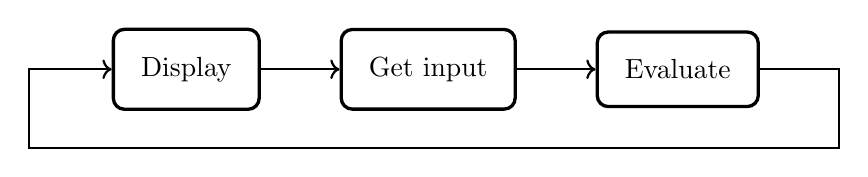
\begin{tikzpicture}
			\tikzset{
				mynode/.style={rectangle,rounded corners, draw=black, very thick, inner sep=1em, text centered},
				usernode/.style={rectangle,rounded corners, draw=black, very thick, inner sep=1em, text centered, fill=black!10},
				dbnode/.style={cylinder,shape border rotate=90,draw=black, very thick, minimum height=2cm, aspect=0.25},
			}
			\node[mynode] (message) {Display};
			\node[mynode, right = of message] (command) {Get input};
			\node[mynode, right = of command] (process) {Evaluate};

			\draw[->, thick] (message) -- (command);
			\draw[->, thick] (command) -- (process);
			\draw[->, thick] (process.east) -- ++(1, 0) -- ++(0, -1) -| (-2, 0) -- (message.west);
		\end{tikzpicture}
		\caption{Core game loop}
		\label{fig:gameplay}
		\end{figure}

	The game processes the command and replies with a new description, and another prompt. That is the core interface and game play. See Figure \ref{fig:gameplay}:

	\begin{compactitem}
		\item \textbf{Display}: The game presents a block of text
		\item \textbf{Get input}: User types in a command
		\item \textbf{Evaluate}: Game engine processes the incoming command, updating the game state
	\end{compactitem}
\end{homeworkSection}


\begin{homeworkSection}{Game Objects}
	There are four types of objects in the COAL engine:
	\begin{compactitem}
		\item \textbf{Rooms}: The locations inhabited by the player characters
		\item \textbf{Items}: Objects the player character interact with such as boxes, lanterns, weapons, etc.
		\item \textbf{Characters}: The internal representation of a user's character, capturing the game state
		\item \textbf{Events}: How the game engine responds to user commands
	\end{compactitem}

\begin{table}
	\begin{tabularx}{\textwidth}{|r|X|}
		\hline
		Property & Description \\
		\hline \hline
		Title & Short name for a room, e.g. \texttt{Forest} \\
		Description & Longer text with details of what the room looks like \\
		Exits & A list of visible directions mapped to destinations, e.g. \texttt{East $\rightarrow$ House} \\
		\hline
	\end{tabularx}
	\caption{Room properties}
	\label{tab:room-properties}
\end{table}

\begin{table}
	\begin{tabularx}{\textwidth}{|r|X|}
		\hline
		Property & Description \\
		\hline \hline
		Name & Short name for the item, e.g. \texttt{Sting} \\
		Aliases & Other words that can be used for the item, e.g. \texttt{sword} \\
		Description & Additional details, e.g. \texttt{An Elvish short-sword that is somewhat fond of spiders} \\
		Properties & A dictionary of key--value pairs for metadata (for example, to track the number of times a potion can be used, and item might have: \texttt{doses} $\rightarrow$ \texttt{5}) \\
		Location & Current room the object is in (or none, if it's inside something else or in a player's inventory) \\
		\hline
	\end{tabularx}
	\caption{Item properties}
	\label{tab:item-properties}
\end{table}

\begin{table}
	\begin{tabularx}{\textwidth}{|r|X|}
		\hline
		Property & Description \\
		\hline \hline
		Name & In--game name of the player character \\
		Player & User account the character belongs to \\
		Location & Room where the character is located \\
		Inventory & Items acquired by the player character \\
		Properties & A dictionary of key--value pairs for storing game state (e.g. \texttt{HAS-SEEN-WELCOME-TEXT} $\rightarrow$ \texttt{TRUE}) \\
		\hline
	\end{tabularx}
	\caption{Character properties}
	\label{tab:character-properties}
\end{table}

\begin{table}
	\begin{tabularx}{\textwidth}{|r|X|}
		\hline
		Property & Description \\
		\hline \hline
		Command & Static text with (optionally) variables describing the syntax of the action. See the \textit{Input Parsing} section for examples. \\
		Conditions & A list of assertions that govern which set of actins should be run in response to command. \\
		True actions & A list of Event Items that manipulates the game state if all of the event conditions are all met, or if there are no event conditions. \\
		False actions & A list of Event Items that manipulates the game state if any of the event conditions are not met. \\
		\hline
	\end{tabularx}
	\caption{Event properties}
	\label{tab:event-properties}
\end{table}

\begin{table}
	\begin{tabularx}{\textwidth}{|r|X|}
		\hline
		Property & Description \\
		\hline \hline
		Primitive & A game engine function. For example, to display a message to the user, the game engine defines a function called \texttt{message}. \\
		Arguments & Arguments to the game engine function. For example, which message to display. \\
		\hline
	\end{tabularx}
	\caption{Event item properties}
	\label{tab:event-item-properties}
\end{table}

	Each of the object types has a number of \textit{properties}. Those properties are either \textit{mutable}, meaning that they can be changed as part of playing the game, or \textit{immutable}. Properties that are immutable can only be edited by game authors outside of the game and cannot be changed through player interactions directly.

	The locations in the game are collectively referred to as ``rooms,'' even though they could be describing outdoor locations, caves, spaceships, or more abstract settings\footnote{For example, \href{https://en.wikipedia.org/wiki/A_Mind_Forever_Voyaging}{A Mind Forever Voyaging} (Infocom, 1985)}. A list of properties is given in Table \ref{tab:room-properties}. When a user enters a room, the full description is shown. A list of directions, like \texttt{NORTH} or \texttt{UP} are mapped against other rooms, connecting them. This list of exits is usable by, and shown to, the player. The title, description, and exits are all immutable properties.

	Items are what users manipulate in the game: weapons, armour, keys, treasure, and so on. The properties of items are given in Table \ref{tab:item-properties}. An item has a name, but also possibly aliases. For example, there may be a book with the name \textit{Hitchhiker's Guide} that also has an alias of \textit{guide}, so the user can type: \texttt{GET GUIDE} or \texttt{GET BOOK} interchangeably. Items may have other attributes, too. For example, if the game has combat elements, then items could have attack or defense values. Last, the only mutable property is the item location, since items can be added to a player character or monster inventory or carried from one room to another and then dropped.

	Table \ref{tab:character-properties} lists the properties of player characters. These are the proxies for users, and so all the state in this object is mutable. Additional properties allow the game engine to track game state. For example, the player character may be poisoned, or under the influence of a potion that lasts for a given number of moves. This key--value mechanism provides an open--ended way to create and manage character data. Each character is associated with one and only one player account, but a player account may have multiple player characters.

	Last, the properties of events are given in Table \ref{tab:event-properties}. The functionality of the game is described using events. All the properties are immutable. The game engine considers each event command string as a pattern -- it will try to match the user input against a single action. Once the engine has has determined which event to execute, all of the conditions for that action are evaluated. If they are all met (or if there are no conditions), then the true actions are evaluated. Otherwise, the false actions are evaluated. The true or false actions dictate actual changes to the state of the game -- moving characters from room to room, manipulating items, and any other game mechanics. The conditions and actions have the same format, given in Table \ref{tab:event-item-properties}. A \textit{primitive} is an actual function in the game engine. Content creators will need to have a list of these functions in order to author the game. The arguments given to the primitives are strings, but can be constants or variable names that are part of the command definition.
\end{homeworkSection}

\begin{homeworkSection}{Creating Game Content}
	Game play requires game content. Classically, in MUDs, once you attained a certain rank within the game\footnote{sometimes called wizard status}, you were allowed to author game content. For some early or small MUDs, this meant recompiling the source code. The prevailing idea, however, was that you could add new content as meta--commands in the game.

	For this project, game content creation is separate from game play, but an integral part of the platform. Users should be able to create rooms, items, monsters, and events. The API is designed with the idea that all game content can be authored in the system. What is exposed from the system is a list of \textit{capabilities} corresponding to the \textit{primitives} discussed in the previous section. Someone designing a MUD should be able to take the exposed functionality and author a complete game. Does the game have a PvP element? It should be programmable enough to allow that. What if there is no combat at all? Or an economy of some sort? It should be possible with the exposed primitives. This places pressure to define a robust set of primitives. I have some ideas, and teams have an opportunity to debate this, but emphasis in the project should be to get the platform working as a whole and not spend excessive time on this until the system is operational as a whole.
\end{homeworkSection}

\begin{homeworkSection}{Design and Architecture Principles}
	\label{sec:design-and-arch}
  Cloud computing is a popular way of deploying large-scale enterprise business applications. Companies large and small outsource their infrastructure and host their applications with cloud computing companies -- be it Amazon, Microsoft, Google, or others. One reason for Amazon's success as a cloud provider is their emphasis on creating \textit{platforms}. The same website that let them sell books became the same one that lets everyone else sell, well, everything. It's a \textit{platform} for online sales. Further, Amazon Web Services (AWS) is consumed by Amazon internally, meaning that the services Amazon sells are the same ones it uses to run their business.
  
  Similarly, the K Division application is a \textit{platform} for MUDs. The game that we should be able to play at the end of this is a \textit{demonstration of the platform} more than a shrink--wrap product\footnote{read more about this here: \url{https://gist.github.com/chitchcock/1281611}}.
  
  The way we build platforms is through \textit{Application Programming Interfaces} (APIs). APIs are everywhere. Google has \href{https://developers.google.com/apis-explorer}{all kinds}. Zoom? They \href{https://marketplace.zoom.us/docs/api-reference/zoom-api}{have an API}. Do you use Slack? They \href{https://api.slack.com/}{have an API} to write bots. So \href{https://developers.facebook.com/}{does Facebook}. Maybe you play games and use Discord. Here's \href{https://discord.com/developers/docs/intro}{their API}.
  
	An \textit{API} is a kind of programming contract. If I provide your service with input that conforms to your specification, then your service agrees to return a result in a given format. For example, an API can be written to accepts and return JavaScript Object Notation (JSON)\footnote{see \href{https://en.wikipedia.org/wiki/JSON}{Wikipedia}} objects. To describe APIs, we are going to use \href{https://swagger.io/specification/}{OpenAPI documents}. OpenAPI is a way of writing descriptions of API contracts in a way that lets us use other code generation software tools to create clients and servers for us.

  You will be given an OpenAPI document that specifies the public--facing API of the COAL Engine. You will negotiate internal APIs with your peer teams. I expect to be able to run a sample game client against this public API and use it to explore your work.
	
	You may want to negotiate changes to the public API, if it doesn't let you fulfill your requirements. Any changes will be discussed in the full class meetings.
\end{homeworkSection}

\begin{homeworkSection}{Application Architecture}
	
\begin{figure}
\centering
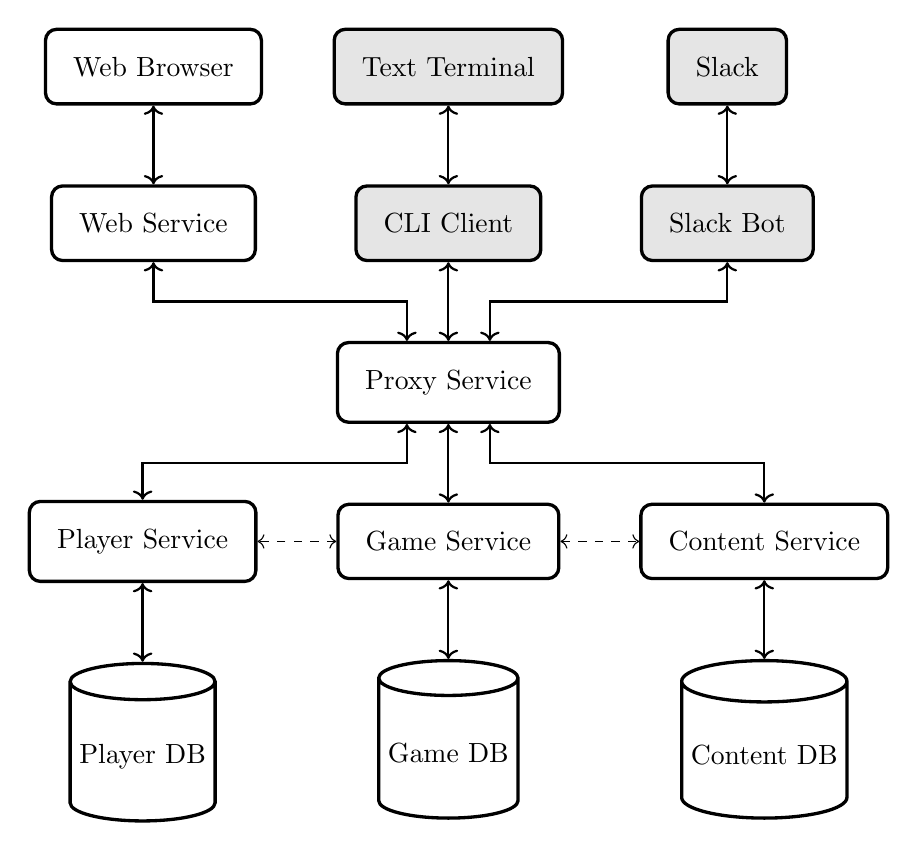
\begin{tikzpicture}
	\tikzset{
    mynode/.style={rectangle,rounded corners, draw=black, very thick, inner sep=1em, text centered},
		usernode/.style={rectangle,rounded corners, draw=black, very thick, inner sep=1em, text centered, fill=black!10},
		dbnode/.style={cylinder,shape border rotate=90,draw=black, very thick, minimum height=2cm, aspect=0.25},
	}
	\node[mynode] (api) at (0,0) {Proxy Service};

	\node[mynode, above left = of api] (webserver) {Web Service};
	\node[mynode, above = of webserver] (webui) {Web Browser};
	\node[usernode, above = of api] (cli) {CLI Client};
	\node[usernode, above = of cli] (term) {Text Terminal};

	\node[usernode, above right = of api] (bot) {Slack Bot};
	\node[usernode, above = of bot] (slack) {Slack};
	\draw[<->, thick] (bot) -- (slack);
	\draw[<->, thick] (bot.south) -- ++(0, -0.5) -| (api.45);

	\draw[<->, thick] (webui) -- (webserver);

	\draw[<->, thick] (cli.south) --  (api.north);
	\draw[<->, thick] (cli.north) --  (term.south);
	\draw[<->, thick] (webserver.south) -- ++(0, -0.5) -| (api.135);

	\node[mynode, below = of api] (gs) {Game Service};
	\node[mynode, left = of gs] (ps) {Player Service};
	\node[mynode, right = of gs] (cs) {Content Service};

	\draw[<->, thick] (api.225) -- ++(0, -0.5) -| (ps.north);
	\draw[<->, thick] (api.south) -- (gs.north);
	\draw[<->, thick] (api.315) -- ++(0, -0.5) -| (cs.north);

	\draw[<->, dashed] (gs.west) -- (ps.east);
	\draw[<->, dashed] (gs.east) -- (cs.west);

	\node[dbnode, below = of gs] (gdb) {Game DB};
	\node[dbnode, below = of ps] (pdb) {Player DB};
	\node[dbnode, below = of cs] (cdb) {Content DB};

	\draw[<->, thick] (gs.south) -- (gdb.north);
	\draw[<->, thick] (ps.south) -- (pdb.north);
	\draw[<->, thick] (cs.south) -- (cdb.north);
\end{tikzpicture}
\caption{Overall Application Architecture}
\label{fig:arch}
\end{figure}

The overall application architecture is given in Figure \ref{fig:arch}. The class is responsible for implementing all of the services shown, while the \textit{Command Line Interface (CLI) Client} is provided. The third--party \textit{Slack} integration is a secondary objective.

The application consists of the following layers:

\begin{compactitem}
	\item \textbf{Presentation Layer}: This layer, consisting of all of the Services and clients above the Proxy service, implement the functionality that lets users play and create content for COAL Engine games. The Web Service makes public API calls into the Proxy Service and presents the results to the user.
	\item \textbf{Application Logic}: The Proxy service brokers requests to the public API, translating them into calls into the other services. It exposes the public API, as given in the OpenAPI specification. The Player service provides user and player character support functions. The Game service implements the core game play loop, evaluating user input and calling into the other services to update game state and provide content. The Content service manages game assets such as room and item descriptions, as well as the other properties associated with them.
	\item \textbf{Data Layer}: The player, game, and content services manage their respective portions of the COAL engine. Since each of these services have different responsibilities, they each have their own databases and associated schemas.
\end{compactitem}

The components of the system are described below, beginning with the REST API itself.
\end{homeworkSection}


\begin{homeworkSection}{Public REST API}
	A REST\footnote{see: \url{https://en.wikipedia.org/wiki/Representational_state_transfer}} API is a way of describing objects and operations against them. A reasonable set of design principles for REST is \href{https://restfulapi.net/}{given here}. In brief, the API has as set of \textit{resources}, or objects in the system, and \textit{methods} used to manipulate them.

	The COAL public API is given in the API Specification PDF. Each URL endpoint is given, along with the expected input parameters, HTTP verb (GET, POST, PUT, or DELETE),  response code (e.g. 200, 201, 404) and output format. All data is transferred via JSON documents.

	For example, a \textit{game} is a resource. Each instance of the \textit{game} resource can be completely different -- different game logic, different rooms and items. Having different games is how COAL is a platform instead of just a game engine.

	To list all of the available games available in the COAL application, the \texttt{/game} endpoint is used with the HTTP \texttt{GET} verb. For example, consider a Proxy service that is listening to port 8100 on the local machine. Using the \href{https://curl.se/}{cURL} tool, the list of games can be retrieved, for example:

\begin{Verbatim}[fontsize=\small]
; curl -X GET http://localhost:8100/v1/game
[
  {
    "id": "7c6b1fc3-0919-495c-bc80-dc1a8737a745",
    "title": "undermud"
  }
]
\end{Verbatim}

	A JSON document is returned by the Proxy service. That document is a list of dictionaries. In the one dictionary that was returned, the short title of the game, \texttt{undermud}, was given, along with an internal unique identifier.

	To retrieve the full details for the game, the \texttt{id} is appended to the URL. For example:

\begin{Verbatim}[fontsize=\small]
; curl http://localhost:8100/v1/game/7c6b1fc3-0919-495c-bc80-dc1a8737a745
{
  "description": "MUD for all",
  "id": "7c6b1fc3-0919-495c-bc80-dc1a8737a745",
  "properties": {
    "starting-message": "Welcome to UnderMUD!",
    "starting-room": "56065d49-0499-43ec-a0aa-b9e74f91a198"
  },
  "title": "undermud"
}
\end{Verbatim}	

	In the GET call above, the \texttt{id} and \texttt{title} are shown again, along with the long form description and properties.

	Creating a game uses a different HTTP verb: \texttt{POST}. A JSON document needs to be provided that specifies the title and description for the game:

\begin{Verbatim}[fontsize=\small]
; curl -X POST \
       -H 'Content-type: application/json' \
			 http://localhost:8100/v1/game \
			 -d'{"title": "new", "description": "New MUD!"}'
{
  "description": "New MUD!",
  "id": "dd290617-a480-4285-a857-e3312a3be831",
  "properties": {},
  "title": "new"
}
\end{Verbatim}

	In the cURL call, the HTTP verb (\texttt{-X POST}) is specified, that the data is a JSON document (\texttt{-H `Content-type...'}), and the data itself. The Proxy service sends the request to the Game service, which then creates the game and sends the details back. Notice that the \texttt{id} is generated by the Game service.

	Other game objects correspond to sub--resources of the \texttt{/game} endpoint:
	\begin{compactitem}
		\item \texttt{/game/\{game\_id\}/room}: Manipulate rooms; see Table \ref{tab:room-properties}
		\item \texttt{/game/\{game\_id\}/item}: Manipulate items; see Table \ref{tab:item-properties}
		\item \texttt{/game/\{game\_id\}/event}: Manipulate events; see Table \ref{tab:event-properties} and Table \ref{tab:event-item-properties}
	\end{compactitem}
	
	Users have accounts with COAL in the form of player objects. Signing up with the application is a call against the \texttt{/player} endpoint. While characters can be retrieved as a sub--resource: \texttt{/player/\{player\_id\}/character}, creating a character is a function of the game service. 
	
	That is, creating a character is a POST to:
	 
	\texttt{/game/\{game\_id\}/player/\{player\_id\}/character} 
	
	The game service is responsible for creating the character and establishing any initial properties for it.

	To learn about all of the endpoints that the Proxy service must implement, review the API Specification PDF. The specification details all of the JSON documents that are sent and received, including fields names and structures. The specification is also what the game clients (that is, the user--facing web service) must implement in order to properly communicate with the Proxy service.
\end{homeworkSection}

\begin{homeworkSection}{OpenAPI Specification}
	The API Specification PDF that you are given describes the REST API in detail. The text file used to create the PDF is also given to you, and is called \texttt{openapi.yaml}. This file is the OpenAPI document mentioned in the \textit{Design and Architecture Principles} section. The document is a text file in the YAML format; \href{https://en.wikipedia.org/wiki/YAML}{see this page}. Describing APIs in this way lets us use tools to generate code for servers and clients in a large number of languages. These YAML documents are also used in testing services and clients.

	Using the same example as above, retrieving the details of a particular game from the COAL application is described by the following fragment:
\begin{verbatim}
/game/{game_id}:
  get:
    summary: Retrieve game details
    parameters:
      - $ref: '#/components/parameters/gameId'
    responses:
      '200':
        $ref: '#/components/responses/GameDetailResponse'
\end{verbatim}

The path (\texttt{/game}) is first, followed by the HTTP verb: \texttt{get}. The URL parameters are listed after a human--readable description. The \texttt{\$ref} is a \textit{reference} to another part of the document that describes the \texttt{game\_id} identifier.

Expected responses are described starting with their HTTP status code. Since responses can be the same for different operations, describing the response only once avoids errors. The \texttt{\$ref} allows sections of the document to be re--used. The \texttt{GameDetailResponse} contains these details:

\begin{verbatim}
responses:
  GameDetailResponse:
  description: Game detail
  content:
    application/json:
      schema:
        $ref: '#/components/schemas/GameDetail'
\end{verbatim}

The \texttt{content} section shows that the response should be in JSON format, and that it should contain a \texttt{GameDetail} object, shown here:

\begin{verbatim}
GameDetail:
  type: object
  properties:
    id:
      type: string
    title:
      type: string
    description:
      type: string
    properties:
      type: object
      additionalProperties:
        type: string
\end{verbatim}

Finally! The \texttt{GameDetail} object describes the properties that will be returned in the JSON document. Each property (\texttt{id}, \texttt{title}, \dots) has a data type, at a minimum, but more sophisticated definitions are possible (see: \href{https://swagger.io/specification/}{the OpenAPI specification}). Each of these properties lines up with part of the JSON from the example in the previous section.

The OpenAPI YAML file is quite long. The API Specification PDF is meant to help you interpret the specification in terms of the JSON that is sent and received by the services. Additionally, use the tools listed at the end of this document to explore the YAML.

If a team want to propose changes to the public COAL API, then I will work with the team to present the modifications necessary to the OpenAPI document.

\end{homeworkSection}



\begin{homeworkSection}{Web service}
	The web service provides the front--end for the game. Users must be able to manage their account and game characters. They must also be able to play the game itself using an interactive console. While the Web service renders the game output, it uses the public API to communicate with the Proxy service.
\end{homeworkSection}


\begin{homeworkSection}{Proxy service}
	The Proxy service is a bridge between the public API and all of the internal components of the application. It has no direct access to the databases, and does not know how the data is stored. Instead, it accepts incoming requests from users and translates them into messages for the internal services and then sends back properly formatted responses.
	
	This design is a pattern for providing \textit{horizontal scaling}. Multiple Proxy services can be launched to accommodate user load independently of the other services, since those services may themselves have specific ways to manage their resources.

	The Proxy service must send and receive JSON content according COAL public OpenAPI specification.
\end{homeworkSection}

\begin{homeworkSection}{Data model conventions}
	The \texttt{title} data model field is a unique, human--readable, one word \textbf{key}. Think of a \texttt{title} like a hashtag. In contrast, \texttt{description} fields are potentially multi--line text fields with as much text as needed. Properties tables are dictionaries or maps of keys (\texttt{titles}) and values; they're an open--ended mechanism for storing data. Most tables have an \texttt{id} field. This field is a primary key, separate from \texttt{title}.
\end{homeworkSection}

\begin{homeworkSection}{Player service}

\begin{figure}
	\centering		
  \begin{tikzpicture}
    % Entity 1
		\pic {entity={P}{Players}{%
                id \\
                title \\
            }};

		\pic[below = 1.5cm of P] {entity={C}{Characters}{%
                id \\
								game\_id \\
                title \\
            }};

		\pic[right = 1.25cm of C] {entity={S}{Properties}{%
						id \\
						character\_id \\
						title \\
						value \\
				}};

		\pic[left = 1.25cm of C] {entity={I}{Items}{%
				id \\
				character\_id \\
				item\_id \\
		}};

    % Draw the cardinalities
		\draw[cfoneone] (P.south) -- (C.north);
		\draw[cf0many] (C.north) -- (P.south);

		\draw[cfoneone] (C) -- (S);
		\draw[cf0many] (S) -- (C);

		\draw[cfoneone] (C) -- (I);
		\draw[cf0many] (I) -- (C);
		
  \end{tikzpicture}
\caption{Player service data model}
\label{fig:player-db}
\end{figure}
	
	The Player Service is responsible for user accounts and managing the game characters the user creates. Figure \ref{fig:player-db}, shows a basic data model. Players may have multiple characters. Each character has a set of properties and a set of items. The \texttt{item\_id} and \texttt{game\_id} foreign keys belong to the content and game services respectively.

	\end{homeworkSection}

\begin{homeworkSection}{Content Service}

	\begin{figure}
		\centering		
		\begin{tikzpicture}
			% Entity 1
			\pic {entity={I}{Items}{%
									id \\
									title \\
									description \\
									location \\
							}};

			\pic [right = 1.25cm of I] {entity={IA}{ItemAliases}{%
							id \\
							item\_id \\
							title \\
					}};

			\pic [left = 1.25cm of I] {entity={P}{Properties}{%
					id \\
					item\_id \\
					title \\
					value \\
			}};

			\pic[below = of I] {entity={R}{Rooms}{%
									id \\
									game\_id \\
									title \\
									description \\
							}};
	
			\pic[right = 1.25cm of R] {entity={E}{Exits}{%
							id \\
							from\_room\_id \\
							to\_room\_id \\
							direction \\
					}};
	
			% Draw the cardinalities
			\draw[cfoneone] (I) -- (IA);
			\draw[cf0many] (IA) -- (I);

			\draw[cfoneone] (I) -- (P);
			\draw[cf0many] (P) -- (I);

			\draw[cfoneone] (R) -- (E);
			\draw[cf0many] (E) -- (R);
			
		\end{tikzpicture}
	\caption{Content service data model}
	\label{fig:content-db}
	\end{figure}
	
	The Content service contains all of the game assets -- text, descriptions, and properties for rooms and items. Figure \ref{fig:content-db} is a basic data model. Items can have have multiple properties and aliases. An Item \texttt{location} is a \texttt{room\_id}. Rooms can have zero or more exits. The \texttt{Exits} table has two foreign key fields that reference the same table. That is, \texttt{from\_room\_id} and \texttt{to\_room\_id} are both \texttt{room\_id} fields referencing the \texttt{Rooms} table. 
	
	Implied in this schema is that room exits are not reciprocal. That is, just because a character can go \texttt{UP} into a room doesn't mean the character can go back \texttt{DOWN} to where they were.
\end{homeworkSection}

\begin{homeworkSection}{Game Service}
	\begin{figure}
		\centering		
		\begin{tikzpicture}
			% Entity 1
			\pic {entity={G}{Game}{%
									id \\
									title \\
									description \\
							}};

			\pic [right = 1.25cm of G] {entity={P}{Properties}{%
				id \\
				game\_id \\
				title \\
				value \\
			}};

			\draw[cfoneone] (G) -- (P);
			\draw[cf0many] (P) -- (G);

			\pic [below = 1.5 cm of G] {entity={E}{Events}{%
				id \\
				game\_id \\
				command \\
			}};

			\draw[cfoneone] (G) -- (E);
			\draw[cf0many] (E) -- (G);

			\pic[right = 1.25cm of E] {entity={C}{Conditions}{%
				id \\
				event\_id \\
				position \\
				primitive \\
			}};

			\draw[cfoneone] (E) -- (C);
			\draw[cf0many] (C) -- (E);

			\pic[right = 1.25cm of C] {entity={CA}{ConditionArgs}{%
				id \\
				event\_item\_id \\
				position \\
				title \\
			}};

			\draw[cfoneone] (C) -- (CA);
			\draw[cf0many] (CA) -- (C);

			\pic[below = of C] {entity={TP}{TruePart}{%
				id \\
				event\_id \\
				position \\
				primitive \\
			}};

			\draw[cfoneone] (E.300) |- (TP);
			\draw[cf0many] (TP.west) -| (E.300);

			\pic[right = 1.25cm of TP] {entity={TA}{TrueArgs}{%
				id \\
				event\_item\_id \\
				position \\
				title \\
			}};

			\draw[cfoneone] (TP) -- (TA);
			\draw[cf0many] (TA) -- (TP);

		\pic[below = of TP] {entity={FP}{FalsePart}{%
			id \\
			event\_id \\
			position \\
			primitive \\
		}};

		\draw[cfoneone] (E.240) |- (FP);
		\draw[cf0many] (FP.west) -| (E.240);

		\pic[right = 1.25cm of FP] {entity={FA}{FalseArgs}{%
		id \\
		event\_item\_id \\
		position \\
		title \\
		}};

		\draw[cfoneone] (FP) -- (FA);
		\draw[cf0many] (FA) -- (FP);

		\end{tikzpicture}
	\caption{Game service data model}
	\label{fig:game-db}
	\end{figure}

	The Game Service is responsible for managing game play. The service reaches out to the content service for room and item descriptions, and to the player service to fetch and update character data. Figure \ref{fig:game-db} has a basic data model. The game engine parses user input (described in the next section), evaluates events, and returns results back to the user.

	The game engine logic is captured in the \texttt{Events} table and its children. An event has three parts -- conditions to evaluate, steps to follow if those conditions are met, and steps to follow if they do not. All three of these parts consist of ordered lists, and so have a \texttt{position} field. Also, all three of these parts consist of a game engine function, called a \texttt{primitive}, and arguments to that function captured in the \texttt{ConditionArgs}, \texttt{TrueArgs}, and \texttt{FalseArgs} tables.

\end{homeworkSection}

\begin{homeworkSection}{Input Parsing}
	Text adventure games and MUDs have all kinds of ways to understand what the user is trying to do with their characters. Turning user input into actions for the game engine is called \textit{parsing} the input.

	The COAL engine uses a specific parsing algorithm that's not as sophisticated as some\footnote{For example, the parser used by the \href{http://www.tads.org/t2doc/doc/parser.htm}{Text Adventure Development System (TADS)}}, but also not as simple as the ones used in the first text adventure games\footnote{Specifically, the first commercially successful ones published by \href{https://en.wikipedia.org/wiki/Scott_Adams_(game_designer)}{Scott Adams} in 1978, which understood only two words, and only the first three letters of each word at that.}.

	Consider that each \texttt{Event}, as above, has a \texttt{command}. That \texttt{command} is a pattern consisting of words and variables. For example, all of these could be commands in the same game:

	\begin{compactitem}
		\item \texttt{GIVE !ITEM TO !CHARACTER}
		\item \texttt{GIVE !ITEM TO BEAR}
		\item \texttt{GIVE HONEY TO BEAR}
	\end{compactitem}

	In the first command, there are two variables: \texttt{!ITEM} and \texttt{!CHARACTER}. All variables are prefixed with a (\texttt{!}). If the user typed: \texttt{GIVE LANTERN TO WIZARD}, then that would be a valid match for that command. However, if the user typed: \texttt{GIVE FOOD FOR BEAR}, then that wouldn't be understood, because \texttt{FOR} isn't part of any of the command patterns.

	\begin{algorithm}
		\caption{COAL Parser, Part 1}
		\label{alg:coal-part-1}
		\begin{algorithmic}
			\Procedure{FindEvents}{$input$}
				\State $w \gets$ number of words in input
				\State $c \gets$ commands of length $w$
				\For{$i \gets 1,w$}\Comment{Look at each word}
					\State $keepers \gets$ empty list\Comment{Store events that match the input word}
					\For{$r \gets 1,c$}\Comment{Check each event}
						\If{$w[i] = r[i]$ or $r[i]$ is a variable}
							\State $keepers.append(r)$
						\EndIf
					\EndFor
					\State $c \gets$ keepers\Comment{discard events that do not match}
				\EndFor
				\State \textbf{return} $c$\Comment{return all events that match the input}
			\EndProcedure
	\end{algorithmic}
	\end{algorithm}

	The first part of the algorithm is given in Algorithm \ref{alg:coal-part-1}. This part creates list of matching events. First, the database is queried for all events that have commands with the same number of words as the input. Next, each word in the input is evaluated. The input word is compared to the command words, in the same position, and events that match are kept. If the command word is a variable, then it's an automatic match -- any input value is accepted. Otherwise, the input and command words must be the same for a match. Last, only events with matches are kept when looking at subsequent words. Once all of the input words are evaluated, the algorithm returns a list of events that match.
	
	Using the algorithm, and the commands above, if the user typed: \texttt{GIVE LANTERN TO BEAR}, then the first two events would match. The first matches because both variables accept the input, and the second matches because of the \texttt{BEAR} part. The last rule does not match, because the user typed \texttt{LANTERN} and not \texttt{HONEY}.

	If there are no matches on the events, an error is returned. For example, \texttt{I DO NOT UNDERSTAND} could be return as a message to the user.

	If only one event is left, then that event can be evaluated (see the next section on how events are evaluated).

	If multiple rules match, then the most specific one is selected. That is, an algorithm should find the event that has the fewest variables. In the example, that is this rule: \texttt{GIVE !ITEM TO BEAR}, since this has one variable, and the other rule has two (\texttt{!ITEM} and \texttt{!CHARACTER}).

	\begin{algorithm}
		\caption{COAL Parser, Part 2}
		\label{alg:coal-part-2}
		\begin{algorithmic}
			\Procedure{ReduceEvents}{$input$, $events$}
				\State $w \gets$ number of words in input
				\For{$i \gets 1,w$}
					\If{length($events$) $= 1$}\Comment{Is the algorithm done?}
						\State \textbf{return} $events[0]$
					\EndIf
					\State $keepers \gets$ empty list
					\For{$r \gets 1,events$}
						\If{$w[i] = r[i]$}\Comment{Is the input word an exact match?}
							\State $keepers.append(r)$
						\EndIf
					\EndFor
					\If{length($keepers$) $>0$}\Comment{Keep only exact matches, if possible}
						\State $events \gets keepers$
					\EndIf
				\EndFor
				\If{length($events$) $>1$}
					\State \textbf{return} ``Error"\Comment{Input is still ambiguous}
				\EndIf
				\State \textbf{return} $events[0]$
			\EndProcedure
		\end{algorithmic}
	\end{algorithm}

	Algorithm \ref{alg:coal-part-2} filters the events from Part 1. Again, this algorithm searches word by word through the user input. All the rules will match -- but if there's a word that matches \textit{exactly} then that event is kept. At the end of the inner loop through all of the events, one of two things is true: (a) there is a set of events with exact matches, or (b) that particular word is a variable in all events. If (a) is true, then the set of events to process \textit{becomes} the set of matched events. Otherwise, the algorithm continues onto the next input word.

	At any time, if only one event remains, then the algorithm stops and returns that event. If, at the end of the algorithm, there are still multiple matches, then this represents a problem with the rules themselves -- an ambiguity has been created. The program shouldn't crash at this point, though, but rather return an error.

	One an event has been found, it is evaluated. This evaluation can change game state and produces an output message for the user. The next section details this process.

\end{homeworkSection}

\begin{homeworkSection}{Game Engine Primitives}
	Once user input is parsed and an event identified, it is evaluated. Game authors need to have the ability to make the game respond to commands, and the facility for this is another API. This API manipulates game state, but not content. That is, the API can set properties, but not change room descriptions.

	The API consists of functions and arguments to those functions in the game engine. Arguments can be constant strings or command variables.

	\begin{table}
		\begin{tabularx}{\textwidth}{|r|l|X|}
			\hline
			Primitive & Arguments & Description \\
			\hline \hline
			is\_property\_eq & key, value & Is the character property \textit{key} equal to \textit{value} \\
			is\_property\_gt & key, value & Is the character property \textit{key} greater than \textit{value} \\
			is\_property\_lt & key, value & Is the character property \textit{key} less than \textit{value} \\
			\hline
		\end{tabularx}
		\caption{Event condition primitives}
		\label{tab:event-condition-primitives}
	\end{table}

	There are two classes of functions -- conditions, and actions. Conditions are used to evaluate the game state. For example, \texttt{is\_property\_eq(key, value)} asks whether the value of character property \texttt{key} matches an argument. Each condition has a boolean result. A list of condition primitives is given in Table \ref{tab:event-condition-primitives}.
	
	The first part of evaluating an event is to evaluate all of its conditions. If all of its conditions are true, then the list of true actions are run (see Table \ref{tab:event-item-properties}). An event may also have \textit{no} conditions, in which case the true actions are run automatically. Otherwise, if any condition is false, then the false actions are run.

	A user can issue a command, have it recognized by the engine, but still result in some error message because of how the event conditions were evaluated. This is perfectly reasonable -- \texttt{GIVE HONEY TO BEAR} shouldn't result in a successful result if, for example, the \texttt{BEAR} is not present or the character is not carrying \texttt{HONEY}.

	\begin{table}
		\begin{tabularx}{\textwidth}{|r|l|X|}
			\hline
			Primitive & Arguments & Description \\
			\hline \hline
			message     & key        & Send the value of global property \textit{key} to the user \\
			set\_key    & key, value & Set character property \textit{key} to \textit{value} \\
			append\_key & key, value & Add \textit{value} to the end of the existing value of \textit{key} \\
			look        & none       & Send a message with the the title, description, list of exits, and items of the character's current room \\
			\hline
		\end{tabularx}
		\caption{Event action primitives}
		\label{tab:event-action-primitives}
	\end{table}

	An action affects the game state. For example, \texttt{message(key)} sends the value of the game property \texttt{key} back to the user. Some actions are given in Table \ref{tab:event-action-primitives}.

	Lastly, there is one set of events that are always evaluated. Events may have a command string that is empty. These are global events that run for every character on every input. An example of this is displaying a welcome message to new characters. A global event is defined that checks to see if the \texttt{first-time} key is set for a character. If it is, then nothing happens (the \texttt{true\_part} is empty). If it isn't set, then: (a) the welcome message is sent, and (b) the \texttt{first-time} key is set.
\end{homeworkSection}


\begin{homeworkSection}{Secondary Objectives}
	There are things missing from this specification. If we get to them, then these would be interesting:
	\begin{compactitem}
		\item \textbf{Engine Primitives}: The lists of actions and conditions is most likely entirely incomplete. I haven't thought enough about authoring a game to work through what a \textit{minimal} set looks like, so I've taken some guesses. If we get to the point of actually getting game content together then it'll make for some good discussion.
		\item \textbf{Access Control}: Content creation is normally reserved for the people running the game and their designates. The services should be extended to recognize different user access levels -- player and admin, and restrict all of the content creation endpoints to be admin-only.
		\item \textbf{Non--Player Characters (NPCs)}: A feature of some MUDs are monsters and combat mechanics. Sometimes, there are shop and equipment buying mechanics, too. While this might be possible using item objects, having NPCs as their own content type might be easier.
		\item \textbf{Third Party Integration}: The power of having a proxy service is in being able to integrate with other text platforms. For example, a bot could be written that facilitates playing COAL Engine games in Slack or Discord.
	\end{compactitem}
\end{homeworkSection}

\end{homeworkProblem}


%----------------------------------------------------------------------------------------
%	Problem description
%----------------------------------------------------------------------------------------
\begin{homeworkProblem}[Tools and Technology]

	\begin{homeworkSection}{Implementation Language and Environment}
		What language the services are written in and the tools you use to do that are up to you and your team. Different teams may use different languages.
		
		For what it's worth, however, there is a proof of concept implementation written for this project and it:
		\begin{compactitem}
			\item was written entirely in Python,
			\item used SQLite as a database backend,
			\item lived on a Microsoft Surface Pro 6 running Windows 10,
			\item ran on Windows Subsystem for Linux v2 (Ubuntu),
			\item was debugged in Visual Studio Code.
		\end{compactitem}
	\end{homeworkSection}

	\begin{homeworkSection}{Hosting}
		Standing up the application and seeing it work over the Internet makes all of this seem more real. Depending on the technology stack your team chooses, there are different places where you can host it for no cost. A caveat: while the services that you'd want to use are \textit{free}, the company may still want a credit card to be able to sign--up.

		For example, if you want a plain Linux server, then a cloud--based virtual machine (compute instance) would work:
		\begin{compactitem}
			\item Amazon Web Services (\url{https://aws.amazon.com/free}) has a 12 Month Free EC2 compute instance option with 750 hours (roughly a month)
			\item Oracle Cloud (\url{https://www.oracle.com/ca-en/cloud/free}) has an always--free tier with 2 small Linux instances
		\end{compactitem}

		You could use an app hosting service, like Heroku (\url{https://www.heroku.com/pricing}); the free option would also be fine for this course.
	\end{homeworkSection}

	\begin{homeworkSection}{OpenAPI}
		To edit or visualize the COAL specification YAML file, use this site: \url{https://editor.swagger.io/}

		The full specification for what OpenAPI is can be found \href{http://spec.openapis.org/oas/v3.0.3}{here}. We are using v3.0.3. A more easily browsable version is \href{https://swagger.io/specification/}{on this site}. Finally, if you want a friendlier explanation of the specification, \href{https://swagger.io/docs/specification/basic-structure/}{go here}.
	\end{homeworkSection}

	\begin{homeworkSection}{Debugging REST}
		One of the challenges in this project will be working with REST servers. Being able to quickly figure out if what you're receiving from the server is correct is going to be important. There are all sorts of tools to help with this -- paid, free, online, offline, \dots

		I like to go with command line tools, and my favourite for this is cURL (\url{https://curl.se/}). It's available for most platforms and can do far more than we'll use here.

		For online options, the \textit{Advanced REST Client} extension for Google Chrome is fairly simple to use. Or maybe \url{https://hoppscotch.io/}.
	\end{homeworkSection}
\end{homeworkProblem}

\end{document}